% Wie werden die Informationen die Benutzer gezeigt und wie können sie diese manipulieren
%\paragraph{}
\begin{flushleft}
Dieses Kapitel verdeutlicht die Gründe, die zu der Entscheidung geführt haben, React als Framework für die Entwicklung der Benutzeroberfläche zu wählen.
\\
Nachdem die Projektanforderungen definiert wurden, wurden die JavaScript Framework Angular, Vue und React, als Option für die Entwicklung der Benutzeroberfläche bewertet.
\\
Die Kriterien, die berücksichtigt wurden, waren:

\begin{itemize}
  \item
  Die Lernkurve. Der Schwierigkeitsgrad, um das Framework zu lernen.
  
  \item 
  Die Flexibilität des Frameworks.
  Der Zwang, Probleme auf eine bestimmte Weise zu lösen, oder die Alternative, eigene Lösungswege zu finden.
  
  \item 
  Anzahl der Nutzer in den letzten Jahren.
  
  \item 
  Anzahl der ungelösten Probleme (open issues).
  
  \item 
  Statistiken von heruntergeladene NPM-Paketen.
  
  \item 
  Akzeptanz bei den Entwicklern auf Github und StackOverflow.

  \item
  Persönliche Präferenz und Vorkenntnisse des Entwicklungsteams.
\end{itemize}

\end{flushleft}

%HIER KÖNNTEN NOCH DIE STATISTEN, DIE DIE POPULARITÄT JEDEN FRAMEWORK PASSEN
\begin{flushleft}
\textbf{Developer Survey 2021 - StackOverFlow}\\
StackOverFlow ist die größte Gemeinschaft von Softwareentwicklern, die Wissen und Fragen zur Softwareentwicklung austauschen.

Seit 2011 führt StackOverFlow eine Umfrage zur Softwareentwicklung durch.
\end{flushleft}

\begin{figure}
  \centering
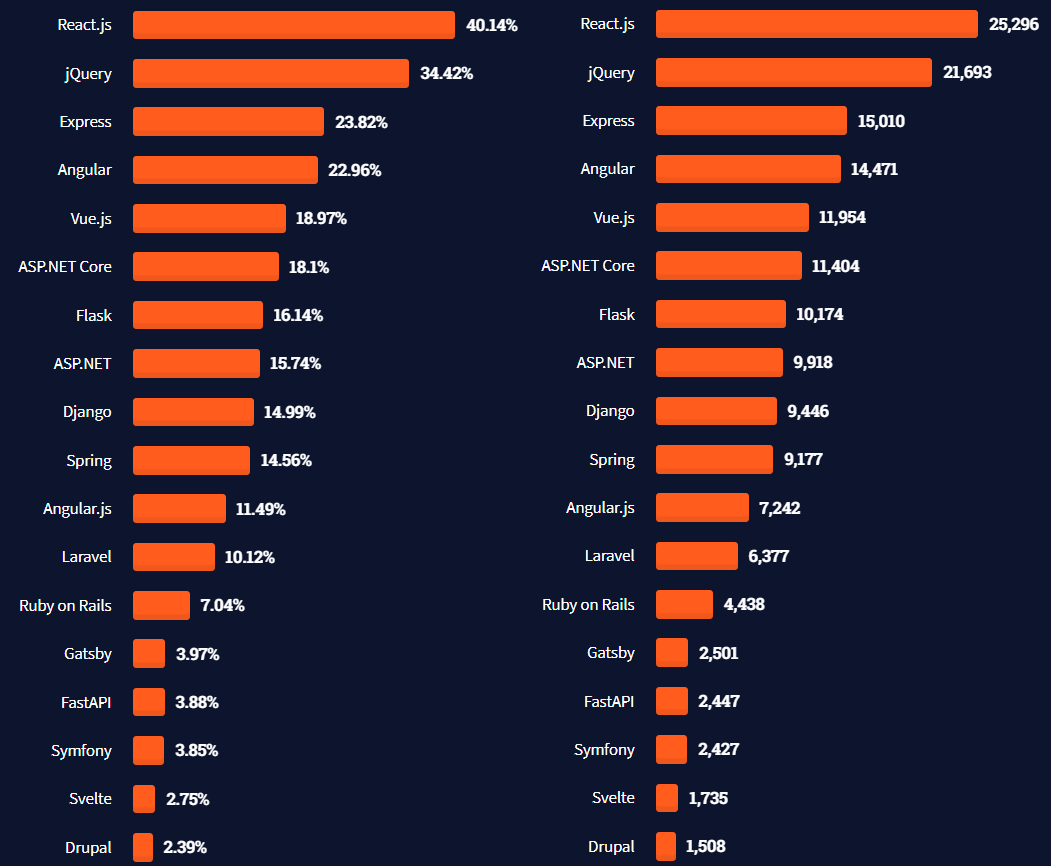
\includegraphics[scale=0.6]
{Most popular Web Frameworks [Both] 2021.png}
    \caption{ Which web frameworks and libraries have you done extensive development work in over the past year, and which do you want to work in over the next year? (If you both worked with the framework and want to continue to do so, please check both boxes in that row.) {\cite{SO01}}}
    
  \end{figure}

 
 
  \newpage
\begin{flushleft}
\textbf{Github}\\
GitHub ist eine webbasierte Schnittstelle, die Git verwendet, die Open-Source-Software zur Versionskontrolle, mit der mehrere Personen gleichzeitig separate Änderungen an Software-Projekte vornehmen können.
\end{flushleft}

Die Anzahl der Repositories, in denen Code für Angular, React und Vue gespeichert ist, gibt einen Hinweis auf die Beliebtheit dieser Frameworks.
\\
\begin{table}[h!]
  \centering
\begin{tabular}{ |p{3cm}||p{3cm}|p{3.6cm}|p{3.6cm}|  }
  \hline
  \multicolumn{4}{|c|}{Github Statistiken}                                                   \\
  \hline
  &@angular/core & Vue & React  \\
  \hline
  Anzahl von Repositories& 2,011,663 & 2,299,614 & 7,868,546
  \\
  \hline
  Offene Issues& 1,716 & 321 & 634
  \\
  \hline
  Stars& 77.2k & 190k & 170k
  \\
\end{tabular}
\end{table}
{\cite{GH01, GH02, GH03}}

%https://risingstars.js.org/2020/es#section-statemanagement
%https://www.freecodecamp.org/news/angular-react-vue/

\textbf{NPM Paketen}\\
NPM verwaltet die Abhängigkeiten eines Angular, React oder Vue Projekts.

Die Anzahl der heruntergeladenen NPM-Pakete gibt einen Hinweis auf die Nutzung der Frameworks.

\begin{center}
  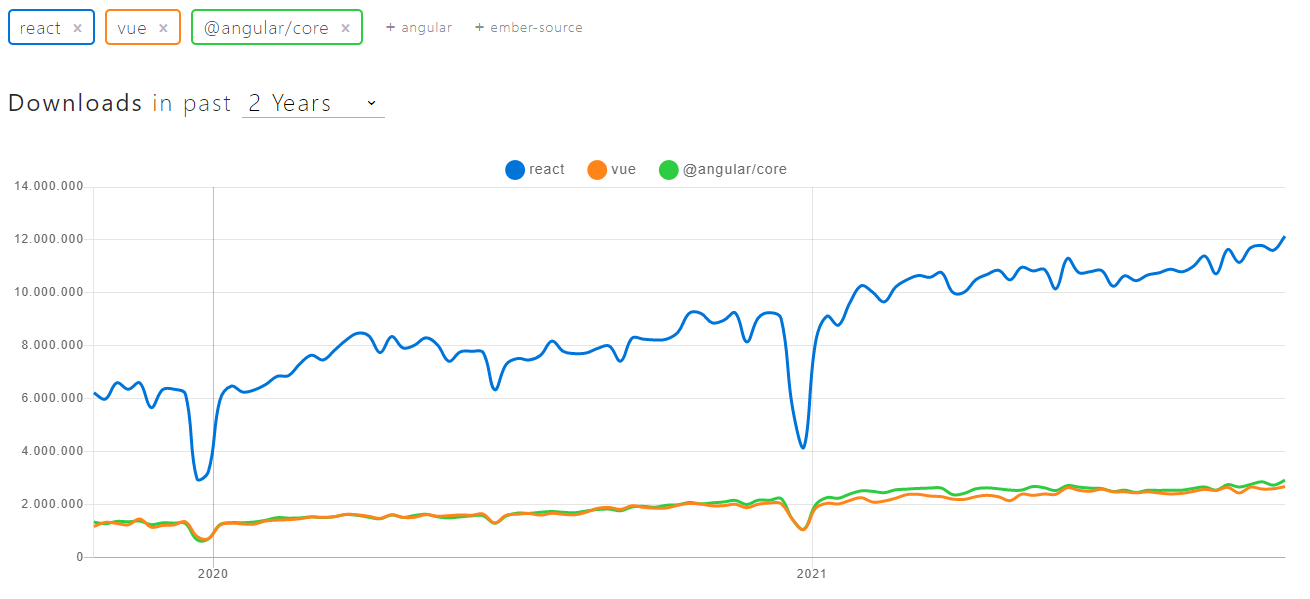
\includegraphics[scale=0.5]{sources/NPM-Trends React_Angular_Vue}\label{fig:NPM-Trends React_Angular_Vue}\\
  \textbf{Abbildung \autoref{fig:NPM-Trends React_Angular_Vue}:} heruntergeladenen NPM-Pakete @angular/core vs react vs vue
  {\cite{NPM01}}
\end{center}

\textbf{Google Trends}\\
Laut Google Trends war React im letzten Jahr das am häufigsten konsultierte Framework in Deutschland. 
Die Daten beziehen sich auf den Zeitraum vom 1.11.2020 bis 26.10.2021.
\begin{center}
  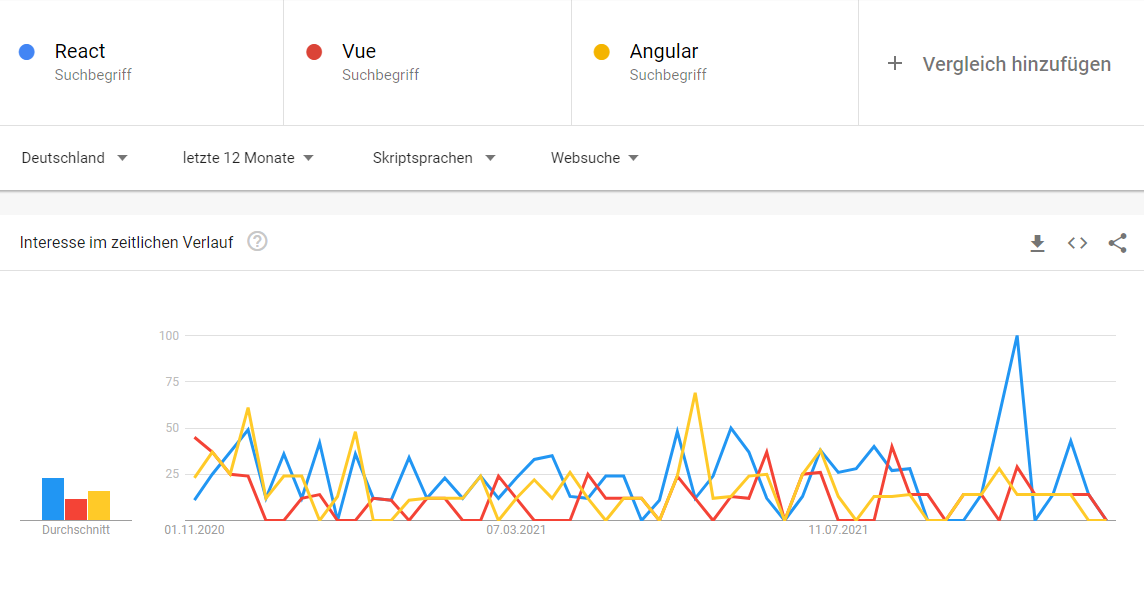
\includegraphics[scale=0.5]{sources/GoogleTrends Vue React Angular 1.11.2020 26.10.2021}\label{fig:GoogleTrends Vue React Angular 1.11.2020 26.10.2021}\\
  \textbf{Abbildung \autoref{fig:GoogleTrends Vue React Angular 1.11.2020 26.10.2021}:} Google Trends Angular vs React vs Vue
  {\cite{GO01}}
\end{center}

\subsection{Angular}
Angular ist das TypeScript Entwicklungsplattform von Google für die Entwicklung von Webanwendungen. 

Die Entscheidung fiel gegen Angular aus den folgenden Gründen:
\begin{itemize}
\item
    Angular ist ein komplexeres Framework als React und Vue.
\item
    Angular ist für Unternehmensanwendungen geeignet. 
\item
    Angular hat eine steile Lernkurve im Vergleich zu React und Vue.{\cite{E01}}
\item
    Angular lässt weniger Spielraum für eigene Entscheidungen darüber, wie der Code entwickelt wird. Deshalb eignet es sich gut für Projekte, bei denen mehrere Entwickler zusammenarbeiten. 
\end{itemize}
\subsection{Vue}

%PASSENTHES KAPITELTHEMA´?

\subsection{Entscheidungsfindung für das Frontend Framework}
Die Entscheidung zwischen Vue und React wurde --TO BE COMPLETED-- wegen ---auch für persönliche Vorlieben und...
\newline
\subsubsection{Vorteile}
\textbf{Deklarativ} \\
Mit React ist es möglich, interaktive Benutzeroberflächen, Ansichten für jeden Zustand der Anwendung zu erstellen. React aktualisiert und rendert effizient genau die richtigen Komponenten, wenn sich deren Daten ändern.
Durch deklarative Ansichten wird der Code vorhersehbarer und einfacher zu debuggen.
\newline

\textbf{Komponentenbasiert}\\
React ist auf gekapselte Komponenten basiert, die ihren eigenen Zustand verwalten.
%Da die Komponentenlogik in JavaScript geschrieben wird, kann man umfangreiche Daten durch die Anwendung leiten und den Zustand aus dem DOM heraushalten.
\newline

\textbf{Große Entwickler-Community}\\
React besteht aus rund 56.162 professionellen Entwicklern auf der ganzen Welt.
Laut einer StackOverFlow Umfrage hat React.js im Jahr 2021 jQuery als das am häufigsten verwendete Web-Framework überholt. {\cite{SO01}}
\newpage

\subsubsection{Nachteile}
Bei der Auswahl des Frameworks wollten wir so unvoreingenommen wie möglich sein, daher listen wir einige Aspekte auf, die bei Projekten mit React zu beachten sind.
\newline

\textbf{JSX}\\
Während dies für einige Entwickler ein Nachteil sein könnte, ist es wichtig zu beachten, dass JSX auch seine Vorteile hat und hilft, den Code vor Injektionen zu schützen.
\newline

\textbf{Ein hohes Entwicklungstempo}\\
Entwickler, die das Entwicklungstempo als Nachteil sehen, würden argumentieren, dass sie die Arbeit mit React ständig neu erlernen müssen und es schwierig ist, damit Schritt zu halten.

Es ist wichtig festzustellen, dass neue Entwicklungen des Frameworks verbessern und dazu beitragen, dass er ein höheres Leistungsniveau erreicht.
\newline

\textbf{Eine zu leichte Dokumentation}\\
Aufgrund der rasanten Entwicklung ist die Dokumentation in Bezug auf die neuesten Aktualisierungen und Änderungen oft spärlich.{\cite{R01}}

\subsection{React Hooks}
\paragraph{}
Beginnend mit 16.8.0, enthält React eine stabile Implementierung von React Hooks. Ab dieser Version wird empfohlen, keine Klassen mehr für die Erstellung von Komponenten zu verwenden.

\subsubsection{useState}
Der Hook useState gibt uns die Möglichkeit, den Zustand unserer Anwendung zu verwalten. Sie besteht aus mindestens einen Wert und einer Funktion, die die besagte Variable aktualisiert.
Der Wert bei der Definition kann ein Zahl, ein String, ein Array oder sogar ein Objekt sein.
Darüber hinaus kann bei der Definition von useState ein Anfangswert festgelegt werden.

\begin{lstlisting}
const [wert, definiereWert] = useState(Anfangswert);
\end{lstlisting}

In unserem Projekt haben wir useState verwendet, um alle damit verbundenen Informationen zu manipulieren und dem Benutzer anzuzeigen.
%\begin{lstlisting}
%    const [profile, setProfile] = useState(state)    
%   \end{lstlisting}

Die Variable state enthält die Daten des angemeldeten Benutzers.
Diese Daten sind die Antwort auf die an den Server gesendete Anfrage.
Ein Beispiel für diese Daten befindet sich im Anhang 1.
\\
In späteren Kapiteln wird näher erläutert, wie diese Informationen, die wir durch einen einzigen Aufruf an den Server erhalten, in den Chat- und Benutzerkomponenten genutzt werden.

Wie man sieht, gibt es innerhalb des states nicht nur einen Wert, sondern mehrere.
Es handelt sich eigentlich um ein Objekt. Objekte sind dasselbe wie Variablen in JavaScript, der einzige Unterschied ist, dass ein Objekt mehrere Werte in Form von Eigenschaften und Methoden enthält.
Objekte können andere Objekte, Strings, Arrays, Zahlen und so weiter enthalten.
\newpage

\subsubsection{useEffect}
useEffect ermöglicht es uns, verschiedene Arten von Effekten zu erzeugen, nachdem eine Komponente gerendert wurde.
\\
\begin{flushleft}
  Der Hook useEffect entspricht einer Kombination aus componentDidMount, componentDidUpdate und componentWillUnmount.

  In unserem Projekt manipulieren wir die Anzeige der Daten abhängig der Änderungen des lokalen Zustands.
\end{flushleft}

Im Zustand „profile“ werden die Änderungen, die der Benutzer an seinen Daten vornimmt, bevor sie in der Datenbank gespeichert werden.
\\
Der globale Zustand „state“ ist in der Komponente App enthalten.
In diesem wird die Antwort von der Datenbankenabfrage gespeichert.
\\
Wir definieren den Zustand als Abhängigkeit von useEffect, so dass er bei jeder Änderung in der Benutzeroberfläche aktualisiert wird.
\\
\begin{lstlisting}
useEffect(() => { 
      setProfile(state)      
  }, [state])           
\end{lstlisting}

\begin{flushleft}
  Es ist möglich, mehrere useEffects zu einstellen und mit ihrer jeweiligen Abhängigkeiten separat definieren.
  Wenn es erfordelich ist, dass der Code innerhalb dem useEffect nur einmal nach dem ersten Rendering ausgeführt wird, muss ein leeres Array als Abhängigkeit definiert werden.
\end{flushleft}
%\newpage

%WELCHES PROBLEM HABEN WIR DAMIT GELÖST?  
\subsubsection{props}
TO COMPLETE/DELETE
\subsubsection{useContext}
useContext hat es uns ermöglicht, Benutzerdaten auf einfache Weise in den Komponenten zu teilen, in denen diese Daten benötigt werden. In frühen Versionen des Projekts wurde für den gleichen Zweck props verwendet.
Unserer Erfahrung nach ist useContext eine elegantere und sauberere Lösung für da gleiche Ziel.
\\
%So funktioniert's
\textbf{useContext Provider} \\
\begin{quote}
  \begin{lstlisting}
    <MyContext.Provider value={/* irgendein Wert */}>
    \end{lstlisting}
  {\cite{R02}}

  %QUE QUIERO DECIR AQUI? Jedes Context-Objekt braucht einen Provider, welcher konsumierenden Komponenten erlaubt, die Veränderungen von Context zu abonnieren.
\end{quote}
Wie der Provider im Projekt definiert wurde ist im Anhang 5 zu finden.

In diesem Fall können die Werte token und state gelesen werden. Darüber hinaus sind die Funktionen setToken, setState und refetch ebenfalls verfügbar.
\\\\
\newpage

\textbf{useContext Consumer} \\
WAS MACHT useContext Consumer?
Code-Auszug in Anhang 6



\subsubsection{Alternative zu useContext}
\paragraph{}
Bei einer früheren Version der kürzlich erläuterten Implementierung haben wir  „props“ verwendet. Dadurch haben wir die gemeinsame Nutzung von Daten zwischen Komponenten ermöglicht. Wir beschlossen, diese Idee zu ändern, da der Code schwieriger zu pflegen war.
\\

\subsubsection{Konklusion}
Es wäre möglich gewesen, das Projekt mit jedem der drei Frameworks durchzuführen.
Die Entwicklung mit Angular hätte mehr Zeit und Lernaufwand gekostet. Außerdem ist das Projekt nicht komplex genug, um das Angular-Ökosystem zu benötigen.
